\documentclass[11pt]{article}
\usepackage[margin=1in]{geometry}
\usepackage[T1]{fontenc}
\usepackage[utf8]{inputenc}
\usepackage{lmodern}
\usepackage{microtype}
\usepackage{amsmath,amssymb}
\usepackage{booktabs}
\usepackage{graphicx}
\usepackage{multirow}
\usepackage{makecell}
\usepackage{xcolor}
\usepackage{pgfplots}
\pgfplotsset{compat=1.17}
\usepackage[numbers,sort&compress]{natbib}
\usepackage[colorlinks=true,linkcolor=blue!50!black,citecolor=blue!50!black,urlcolor=blue!50!black]{hyperref}

\newcommand{\FZ}{\textsf{F0}}
\newcommand{\FO}{\textsf{F1}}
\newcommand{\FZO}{\textsf{F0+F1}}
\newcommand{\Hs}{\textsf{H}}
\newcommand{\ci}[2]{\,[#1,\,#2]}

\title{What the Router Knows:\\Cheap Per-Token Error Detection from Mixture-of-Experts Routing Signals, and Where It Stops Helping}
\author{Mateo Agustin Peralta\\ {Independent researcher}\\ \texttt{map12082004@gmail.com}}
\date{}

\begin{document}
\maketitle

\begin{abstract}
A mixture-of-experts (MoE) language model computes a routing distribution over experts at every layer and every token.
We ask how much these router signals reveal about whether the token being generated belongs to a wrong answer, how they compare with output entropy and with a probe on the hidden state, and what they cost to read in a serving stack.
A linear detector on router statistics (243 for a 24-layer model) and 4 output statistics, calibrated with Platt scaling and thresholded by conformal risk control, has a higher token-level AUROC than output entropy in every factual setting we measured: three MoE models (Granite~3.1~1B-A400M, gpt-oss-20b, OLMoE-1B-7B), Spanish and English questions, and, on gpt-oss, each of the three largest question types.
Where we could run a paired bootstrap, the difference is significant on Granite, in the gpt-oss vLLM run, and on four of the five OLMoE test sets, but not on NQ-Open ($+0.031$, 95\% CI $[-0.004, +0.063]$); for the gpt-oss runs on HuggingFace we have only marginal intervals.
The size of the gain depends strongly on how it is measured.
The headline token-level AUROC of 0.906 on Granite comes from a test set where 92\% of tokens are errors and answer types are confounded with correctness; on 2,600 questions with gpt-oss, pooling the non-arithmetic question types gives 0.723 against 0.556 for output entropy.
The clearest result is per answer: on 1,792 non-arithmetic factual answers, adding router statistics to question type and length raises cross-validated AUROC from 0.679 to 0.811, with a gain in each of the three largest types, while no form of output entropy adds more than 0.03 over length; these are point estimates without intervals.
Router signals stay within 0.02 AUROC of a linear probe on the hidden state, they do not match the published InnerExpert detector on its own protocol (0.651 vs.\ 0.762 average), and on code they mostly act as a tie-breaker.
Their advantage is cost: 4.7\% added latency in HuggingFace on an L4 GPU, and no detectable cost in vLLM, where expert identities alone keep much of the within-type signal.
\end{abstract}

\section{Introduction}

Language models state wrong facts fluently, and a system that serves one often needs a signal, available while the answer is generated, that a span is likely wrong~\citep{ji2023survey,huang2025survey}.
Three families of signals compete.
Output-distribution signals (token entropy, negative log-likelihood) are free but weak~\citep{snyder2024early}.
Sampling-based signals such as semantic entropy~\citep{kuhn2023semantic,farquhar2024detecting} and SelfCheckGPT~\citep{manakul2023selfcheckgpt} are stronger but need several generations.
Probes on hidden states are strong and need one forward pass~\citep{azaria2023internal,chwang2024androids,kossen2024semantic,orgad2025llms,obeso2025realtime}, but they require access to dense activations at a chosen layer.

Mixture-of-experts models~\citep{fedus2022switch} expose a fourth source.
At every MoE layer and every token, a router scores all experts and sends the token to the top $k$.
The router logits are small (one number per expert per layer), the model computes them anyway, and in some serving engines the chosen expert indices can be returned with the tokens.
Reading the logits is not always free: fused kernels may never expose them, and our extractor then recomputes them from the input of each MoE block (Section~\ref{sec:method}).
Two recent works show that routing carries information about errors: InnerExpert~\citep{fonseca2026innerexpert} combines expert-usage statistics with hidden-state and attention scores into a per-token detector, and Routing Entropy~\citep{li2026routing} uses the entropy of routing distributions to verify answers on multiple-choice benchmarks.
A third work finds, in vision transformers with routing, that routing entropy adds nothing once output confidence is controlled~\citep{liang2026auditing}.
A fourth compares a router's choices with counterfactual routes of equal compute and finds the router reliable on confident tokens but often wrong on fragile ones~\citep{yoon2026misrouted}, which gives one reason to expect routing to carry information about errors.

This paper reports a measurement program on that question with three emphases that the prior work does not combine.
First, we measure \emph{incremental} value: against output entropy, against a hidden-state probe, against answer length and question type, and within each question type, because routers are known to encode token and part-of-speech identity~\citep{antoine2025pos} and a detector can learn ``this is an arithmetic question'' instead of ``this is an error''.
Second, we use labels that a program computes (exact match against gold aliases, numeric match, unit tests), so that no language model judges another, except in one replication where we follow the published protocol.
Third, we measure the cost of reading the signals in two serving stacks, including under concurrency.

Our findings:
\begin{itemize}
  \item On factual questions, the router detector has a higher AUROC than output entropy in every setting we measured, within the three largest question types, and on every out-of-distribution test set of the InnerExpert protocol (Tables~\ref{tab:granite}--\ref{tab:innerexpert}). A paired bootstrap, available for the Granite, OLMoE and vLLM runs, confirms the difference everywhere except on NQ-Open. The one setting where the router loses is token-level detection on code with a 1B model.
  \item The size of the gain is smaller than headline numbers suggest. Token-level AUROC on a high-prevalence test with confounded answer types overstates it; pooled over the non-arithmetic types of a larger set, the figure is 0.723 (Table~\ref{tab:v2type}).
  \item Per answer, router statistics add 0.13 AUROC over type and length, and 0.11 to 0.21 within each of the three largest types, while output entropy adds 0.005 (Table~\ref{tab:response}, Figure~\ref{fig:response}). These are cross-validated point estimates; their intervals are pending.
  \item A probe on the hidden state is within 0.02 AUROC of the router wherever both ran; semantic entropy with five samples is below the router by point estimate; the router does not reach InnerExpert's published detector on its own protocol.
  \item On code, the token-level detector fails on a 1B model and is modest on gpt-oss-20b; for best-of-$N$ selection, running the visible examples matters more than the router (Table~\ref{tab:bestofn}).
  \item Reading router logits costs 4.7\% latency in HuggingFace on an L4; returning expert indices in vLLM has no cost we could detect, also with 32 concurrent requests (Figure~\ref{fig:latency}).
\end{itemize}

A companion paper studies a different question on the same models: how fine-tuning overwrites facts, and how certainty read from the model can make it selective~\citep{companion2026forgetting}.
One result there bears on this paper, and we report it in Section~\ref{sec:limits}: the router detector flags erroneous tokens during generation, but it does not read how certain the model is of a stored fact.

\section{Related work}
\label{sec:related}

\paragraph{Router signals for error detection.}
The closest work is InnerExpert~\citep{fonseca2026innerexpert}.
It extracts, per token and per layer, router entropy, expert-usage distributions and their Gini and inverse-Herfindahl summaries, expert-output similarity and expert hidden scores, and adds the hidden-state and attention scores of LLM-Check~\citep{sriramanan2024llmcheck}.
Labels come from an LLM judge (GLM-5.1) that marks hallucinated substrings, and models are trained on RealtimeQA~\citep{kasai2023realtimeqa} and tested on a later RealtimeQA window and four other datasets.
With its logistic-regression classifier it reports an average token-level AUROC of 0.762 on OLMoE-1B-7B-0924-Instruct, against 0.639 for logit entropy; on Gemma-4-26B-A4B-it its best classifier (XGBoost) reaches 0.753 and logistic regression 0.725, against 0.541 for logit entropy.
The full detector runs at roughly three times the cost of plain generation.
Our feature set is a subset of the cheap part of theirs (router statistics only, no expert outputs, no hidden or attention scores); we test it on two more MoE families, on Spanish, with computable labels, inside a production serving engine, and we replicate their protocol on OLMoE (Section~\ref{sec:innerexpert}).
Routing Entropy~\citep{li2026routing} aggregates router entropy over deep layers and final tokens and fuses it with output confidence; on OLMoE it reports AUROC 0.655 alone and 0.680 fused, against 0.639 for output confidence, on multiple-choice benchmarks, and it also uses routing entropy as a training regularizer.
We work per token on free-form answers and do not change training.
\citet{liang2026auditing} audit routing entropy in attention-residual vision transformers and find that it does not beat an output-only baseline once confidence is controlled; we include output features in every comparison for the same reason.
Routers are sensitive to part of speech~\citep{antoine2025pos}, which motivates our within-type controls.
\citet{yoon2026misrouted} score each route by the probability it gives the correct next token and find that routing fails mostly on fragile tokens; they improve the router, whereas we only read it.

\paragraph{Hidden-state probes.}
Linear probes on hidden states separate true from false statements~\citep{azaria2023internal}, detect hallucinated tokens in grounded generation~\citep{chwang2024androids}, predict semantic entropy from one generation~\citep{kossen2024semantic}, and locate hallucinated entities in long-form text in real time~\citep{obeso2025realtime}.
Error information concentrates in specific tokens and does not transfer well across datasets~\citep{orgad2025llms}.
Truth has a linear representation that probes and interventions can find~\citep{marks2024geometry}, and contrast-consistent search finds a truth direction without labels~\citep{burns2023discovering}.
Models can be trained to predict whether they know the answer to a question before answering it~\citep{kadavath2022language}, and internal states of the query alone predict the risk of a hallucinated answer~\citep{ji2024llm}.
INSIDE detects hallucinations from the covariance of internal embeddings across several sampled answers~\citep{chen2024inside}, and HaloScope trains a detector from unlabeled generations by estimating a hallucination subspace of the activations~\citep{du2024haloscope}.
We include a hidden-state probe as a baseline in every setting where we can extract it; our question is not whether the router beats the hidden state, but what fraction of the hidden-state signal survives in a representation that is two orders of magnitude cheaper to log and that some serving engines already return.

\paragraph{Output and sampling signals.}
Token probabilities and entropy are the standard white-box baseline~\citep{snyder2024early}.
Semantic entropy clusters sampled answers by meaning~\citep{kuhn2023semantic,farquhar2024detecting}; SelfCheckGPT checks consistency across samples~\citep{manakul2023selfcheckgpt}.
We compare against semantic entropy with five samples in Section~\ref{sec:semantic}.

\paragraph{Token-level labels.}
Token-level hallucination benchmarks rely on human or model annotation of spans~\citep{liu2022token,vazquez2025mushroom}.
Our main labels are coarser: a whole answer is right or wrong, and its label is copied to all its tokens.
This is a limitation we discuss in Section~\ref{sec:labels}; it buys labels without a judge.

\paragraph{Calibration and risk control.}
We calibrate scores with Platt scaling, as described by \citet{guo2017calibration}, and choose flagging thresholds with conformal risk control~\citep{angelopoulos2024conformal}.
Conformal methods also give guarantees at the level of whole outputs: conformal language modeling calibrates when to stop sampling and which answers to reject~\citep{quach2024conformal}, and conformal factuality removes claims until an output is correct with high probability~\citep{mohri2024language}.
Our use is narrower: we control the expected share of erroneous tokens left unflagged, and we make no guarantee about false alarms.

\section{Signals and detector}
\label{sec:method}

\paragraph{Signal tiers.}
For each generated token we extract three tiers of features.
\begin{itemize}
  \item \textbf{\FZ{} (output, 4 features):} entropy over the full vocabulary, negative log-likelihood of the emitted token, top-1/top-2 logit margin, and entropy over the top 20 tokens.
  \item \textbf{\FO{} (router, 9 statistics per MoE layer plus 27 aggregates):} normalized entropy of the router softmax over the $N$ experts; entropy of the renormalized top-$k$ weights; top-$k$ probability mass; the margins $z_1-z_2$ and $z_k-z_{k+1}$ between sorted router logits; whether the top-$k$ set changed from the previous token; and three summaries of causal cumulative expert usage up to the current token (Gini impurity, normalized inverse Herfindahl index, normalized entropy). For each statistic we also take the mean, maximum, and standard deviation across layers. Granite and gpt-oss-20b both have 24 MoE layers, which gives $9\times24+27=243$ router features; OLMoE has 16, which gives $9\times16+27=171$.
  \item \textbf{\Hs{} (hidden state):} the residual-stream vector at depth $\approx0.95L$, used only by the probe baseline (1,024 dimensions for Granite).
\end{itemize}
The detector by default uses \FZO{} (247 features for 24-layer models, 175 for OLMoE).
The usage statistics follow the expert-usage features of InnerExpert~\citep{fonseca2026innerexpert}, computed causally so that the feature at token $t$ uses only tokens up to $t$.

\paragraph{Extraction.}
We read \FO{} with a forward pre-hook on each MoE block.
The hook takes the block's input $x$ and recomputes the router logits $z = W_{\text{router}}x + b$ in float32 with the router's own weights.
Recomputing costs one small matrix product per layer, and it works when a fused kernel never calls the router module, as in gpt-oss-20b with MXFP4 weights.
The hook keeps only the logits of the current step; the reduction to the statistics above runs once per step on the CPU.
\FZ{} is computed from the output logits on their own device.

\paragraph{Reduced tier for serving engines.}
Some engines return the indices of the chosen experts but not the router logits, and return only the top log-probabilities of the output distribution.
For that case we define a reduced tier: \FZ{} computed from the top-20 log-probabilities, plus the usage statistics and route switches, which depend only on expert indices.
Entropy, mass and margin features of the router softmax are not available in this tier.
Section~\ref{sec:latency} measures how much signal it keeps.

\paragraph{Detector.}
The detector is an $\ell_2$-regularized logistic regression on z-scored features, with the regularization strength chosen by cross-validation grouped by question.
Scores are calibrated with Platt scaling on a held-out calibration split.
To turn the calibrated probability into a flag, we choose a threshold $\tau$ by conformal risk control~\citep{angelopoulos2024conformal}: $\tau$ is the largest value whose finite-sample-corrected empirical risk on the calibration split stays below a target $\alpha$, where the risk of a response with errors is the fraction of its erroneous tokens that are not flagged.
The guarantee holds in expectation over exchangeable responses, so one test split can exceed $\alpha$; it controls missed errors, not false alarms.
We calibrate $\tau$ on a grid of $\alpha$ values.
The \emph{recommended} $\alpha$ is the grid value that maximizes the answer-level detection rate minus the answer-level false-alarm rate on the calibration split, with ties broken toward the smaller $\alpha$; the test split plays no part in the choice.

\paragraph{Baselines.}
Every table reports output entropy and token NLL as single-feature detectors trained and calibrated the same way, and, where \Hs{} is available, a logistic probe on the hidden state.
For per-answer analyses we add answer length and question type, because both predict errors without looking inside the model.

\section{Experimental setup}
\label{sec:setup}

\paragraph{Models.}
Granite~3.1~1B-A400M instruct has 24 MoE layers with 32 experts and top-8 routing; we run it in bf16 on a laptop CPU.
No Granite~3.1 technical report is available, so we cite the model card~\citep{granite31card} and the Granite~3.0 report, which describes the model family~\citep{granite2024granite}.
gpt-oss-20b~\citep{openai2025gptoss} has 24 layers with 32 experts and top-4 routing; we run its MXFP4 weights on a Tesla T4 or an L4 GPU in Colab, with \texttt{reasoning\_effort=low}, and score only tokens of the \texttt{final} channel.
OLMoE-1B-7B-0924-Instruct~\citep{muennighoff2025olmoe} has 16 MoE layers with 64 experts and top-8 routing and is used only for the replication in Section~\ref{sec:innerexpert}.

\paragraph{Factual data.}
The base set has 600 questions: 360 Spanish questions from MKQA~\citep{longpre2021mkqa}, stratified by answer type (entity, date, number, number with unit, short phrase), and 240 generated arithmetic questions (80 each of sums, differences and products).
An expanded set has 2,600 questions with the same composition: 600 arithmetic and 2,000 MKQA questions.
Greedy answers are generated up to 24 new tokens for Granite and 256 for gpt-oss.
Code answers (Section~\ref{sec:code}) are generated up to 384 new tokens for Granite and 768 for gpt-oss.

\paragraph{Labels.}
\label{sec:labels}
An MKQA answer is correct if it matches a gold alias exactly, has token F1 $\ge0.5$ with one, or matches a gold number or date; an arithmetic answer is correct if the result is exact.
Each token of an incorrect answer gets label 1, each token of a correct answer label 0.
This label is coarser than a span label: it also marks filler tokens of a wrong answer as errors.
A token-level AUROC under this label therefore measures whether the tokens of wrong answers look different from the tokens of right answers, not whether the detector localizes the wrong span.
Code answers are labeled by running the benchmark's unit tests in an isolated process.
Only the OLMoE replication uses span labels from an LLM judge, following the protocol being replicated.

\paragraph{Splits and statistics.}
Questions are split 60/20/20 into train, calibration and test (360/120/120 for the base set), grouped by question so that no question appears in two splits.
Intervals are 95\% percentile intervals from a bootstrap that resamples questions (2,000 replicas unless stated; 500 for the stratified controls; 1,000 for the OLMoE replication and the vLLM run).
When two detectors are scored on the same test split, we compare them with a paired bootstrap: the AUROC difference is computed on the same resampled questions in each replica.
Our evaluation code computes this difference for every comparator, but the saved reports contain it only for the Granite base set, the OLMoE replication and the vLLM run.
For the gpt-oss runs on Hugging Face we kept only marginal intervals, and we say so wherever we compare them; overlapping marginal intervals are not a test.
Because AUROC does not depend on prevalence but the difficulty of a test set does, we state the share of positive tokens or answers for every result.

\section{Results on factual questions}
\label{sec:factual}

\subsection{Granite on the base set}

Granite answers 16.2\% of the 600 questions correctly: 53.8\% of sums, 38.8\% of differences, 2.5\% of products, and 5.2\% of MKQA entity questions.
Its test split has 1,035 tokens from 120 answers; 92.1\% of tokens and 83.3\% of answers are errors.
Table~\ref{tab:granite} shows the token-level results.

\begin{table}[t]
\centering
\small
\caption{Granite~3.1~1B-A400M, base set, token-level AUROC on the test split (1,035 tokens, 120 answers; 92.1\% of tokens are errors). AUPRC is reported because the base rate is high; a random detector has AUPRC 0.921.}
\label{tab:granite}
\begin{tabular}{lccc}
\toprule
Detector & Features & AUROC [95\% CI] & AUPRC \\
\midrule
Output entropy & 1 & 0.601\ci{0.547}{0.649} & 0.948 \\
Token NLL & 1 & 0.599\ci{0.543}{0.650} & 0.946 \\
\FZ{} & 4 & 0.644\ci{0.592}{0.695} & 0.952 \\
\FO{} (router only) & 243 & 0.891\ci{0.808}{0.969} & 0.989 \\
\FZO{} (default) & 247 & 0.906\ci{0.830}{0.980} & 0.990 \\
Hidden-state probe & 1,024 & 0.906\ci{0.830}{0.979} & 0.989 \\
\FZO{} + \Hs{} & 1,271 & 0.926\ci{0.865}{0.985} & 0.992 \\
\bottomrule
\end{tabular}
\end{table}

The router lifts AUROC from 0.60 to 0.89; output features add little on top of it.
The paired difference between the default detector and output entropy is $+0.305$\ci{+0.216}{+0.386}.
Per answer (the maximum token score of each answer), the gap is smaller and not significant: 0.894 against 0.845, a paired difference of $+0.049$\ci{-0.035}{+0.126}.
The hidden-state probe matches the default detector exactly (0.906; paired difference $0.000$\ci{-0.032}{+0.036}), so we find no evidence that the router carries information that the late hidden state lacks; it carries what it has in 243 features rather than a 1,024-dimensional vector.
The default detector is well calibrated on test (ECE 0.029\ci{0.016}{0.057}, Brier 0.046).
At $\alpha=0.1$, the mean per-answer miss rate on test is 0.105 and the pooled token miss rate 0.044, with 91.1\% of tokens flagged and token precision 0.966.
The per-answer miss rate is slightly above $\alpha$, which the guarantee allows on a single test split of 100 answers with errors.
The high flag rate mirrors the base rate: the model is wrong on almost everything, and at this prevalence a high AUROC does not make the flags useful by itself.
The 92\% prevalence and the 120-answer test also explain the wide intervals.

\subsection{Confounding by question type}

Arithmetic questions are answered correctly far more often than MKQA questions, and their tokens (digits, operators) route differently.
A detector could learn the question type instead of the error.
To test this, we retrain and evaluate the detector within each stratum (Table~\ref{tab:strata}).

\begin{table}[t]
\centering
\small
\caption{Granite, detector retrained and evaluated within each question stratum (500 bootstrap replicas). Token counts and prevalence (the share of error tokens) are over all generated tokens of the stratum, in all three splits; the AUROCs are on the stratum's test split.}
\label{tab:strata}
\begin{tabular}{lcccccc}
\toprule
Stratum & Prevalence & Output entropy & \FZ{} & \FO{} & \FZO{} & \Hs{} probe \\
\midrule
Arithmetic (853 tokens) & 65.4\% & 0.779 & 0.809 & 0.838 & 0.883 & 0.880 \\
MKQA (4,384 tokens) & 97.3\% & 0.654 & 0.641 & 0.859 & 0.882 & 0.886 \\
\bottomrule
\end{tabular}
\end{table}

Within MKQA, the router's AUROC exceeds output entropy's by more than 0.2.
Within arithmetic, the advantage is smaller (0.883 against 0.779) and the marginal intervals overlap; we did not save a paired test for the strata.
The MKQA stratum has very few correct answers, so its interval is wide.
The result says that the router signal is not only a topic detector on this set, but it does not say how large the gain is on a set with a realistic mix of right and wrong answers.
The next two subsections address that.

\subsection{gpt-oss-20b on the base set}

gpt-oss-20b answers 54.3\% of the same 600 questions correctly, so the classes are more balanced.
Its test split has 914 tokens from 112 answers, with 80.4\% error tokens.

\begin{table}[t]
\centering
\small
\caption{gpt-oss-20b on the base set (Tesla T4). Left: token-level AUROC on the test split (914 tokens, 112 answers; 80.4\% error tokens). Right: detector retrained within each stratum (500 replicas).}
\label{tab:gptoss}
\begin{tabular}{lc@{\hspace{2em}}lccc}
\toprule
Detector & AUROC [95\% CI] & Stratum & Entropy & \FO{} & \FZO{} \\
\midrule
Output entropy & 0.643\ci{0.565}{0.702} & Arithmetic & 0.625 & 0.969 & 0.983 \\
Token NLL & 0.637\ci{0.560}{0.697} & MKQA & 0.552 & 0.834 & 0.837 \\
\FZ{} & 0.650\ci{0.576}{0.705} & Products only & 0.605 & 0.941 & 0.976 \\
\FO{} & 0.875\ci{0.778}{0.947} & Entities only & 0.555 & 0.898 & 0.898 \\
\FZO{} & 0.881\ci{0.783}{0.951} & & & & \\
\Hs{} probe & 0.871\ci{0.753}{0.963} & & & & \\
\FZO{} + \Hs{} & 0.903\ci{0.796}{0.970} & & & & \\
\bottomrule
\end{tabular}
\end{table}

The pattern repeats (Table~\ref{tab:gptoss}): the router lifts AUROC from 0.64 to 0.88, with marginal intervals that do not overlap, and the point estimates keep the gain within one operation (products) and one answer type (entities).
We have no paired test for this run.
The within-stratum intervals are wide: the products stratum has 24 test answers and the entity stratum 60; the MKQA interval for \FO{} is $[0.626, 0.915]$.

\subsection{gpt-oss-20b on 2,600 questions}

On the expanded set, gpt-oss answers 45.7\% correctly: almost all arithmetic and 29.9\% of entity questions.
The test split has 478 questions and 5,320 tokens, 78.3\% of them errors.
The default detector reaches 0.773\ci{0.662}{0.897}, the hidden-state probe 0.793\ci{0.675}{0.909}, and output entropy 0.569\ci{0.528}{0.613}; only these marginal intervals were saved.

The test split contains no arithmetic errors, so the global AUROC again mixes question type with error.
Table~\ref{tab:v2type} breaks it down by type.

\begin{table}[t]
\centering
\small
\caption{gpt-oss-20b, 2,600-question set, token-level AUROC by question type on the test split (point estimates; no intervals were saved). We did not record output entropy for the two small types. The number-with-unit token count is derived as 5,111 minus the other four types. The last row pools all non-arithmetic types.}
\label{tab:v2type}
\begin{tabular}{lccc}
\toprule
Type & Tokens & \FZO{} & Output entropy \\
\midrule
Date & 618 & 0.776 & 0.592 \\
Entity & 3,912 & 0.689 & 0.544 \\
Number & 119 & 0.634 & 0.494 \\
Short phrase & 187 & 0.27 & -- \\
Number with unit & 275 & 0.97 & -- \\
All except arithmetic & 5,111 & \textbf{0.723} & 0.556 \\
\bottomrule
\end{tabular}
\end{table}

The router's point estimate exceeds output entropy's in each of the three largest types, but the pooled non-arithmetic number is 0.72, not the 0.77 of the global test or the 0.88 of the 600-question run.
The two small types give unstable values: on short phrases (187 tokens) the detector is inverted (0.27), and on numbers with units (275 tokens) it reaches 0.97; we do not interpret either.
We regard 0.72 against 0.56, pooled over the non-arithmetic types, as the best single estimate of the token-level gain of the router on factual questions for this model.

Per answer, a flagging rule maps the token threshold to an answer flag when any token is flagged.
The $\alpha$ recommended on the calibration split (0.26; Section~\ref{sec:method}) flags 86\% of wrong answers with 27\% false alarms on test (241 wrong and 237 right answers); $\alpha=0.42$ flags 76\% with 16\% false alarms (Appendix~\ref{app:pareto}).
These rates do not control for type.
All 241 wrong answers are non-arithmetic, while 127 of the 237 right answers are arithmetic: the test split has 478 answers, 351 of them non-arithmetic, and no arithmetic errors.
We did not save per-type answer flags, so the false-alarm rate on the 110 right non-arithmetic answers is unknown; if the 64 false alarms fell mostly on them, it would be as high as 58\%.

\subsection{Per answer: the router beyond type and length}
\label{sec:response}

The token-level label is coarse, and question type is a confound.
The cleanest test of the router is therefore per answer, with type and length as covariates.
We take the 1,792 non-arithmetic answers of the 2,600-question run (67\% wrong) and compare cross-validated logistic models (Table~\ref{tab:response}).
The other 208 of the 2,000 non-arithmetic answers have no scored token in the \texttt{final} channel or no computable label, so they have no features.
Each question has one answer, so the five stratified folds also split questions.

\begin{table}[t]
\centering
\small
\caption{gpt-oss-20b, per-answer AUROC on 1,792 non-arithmetic answers (67\% wrong); point estimates without intervals. ``CV'' rows are 5-fold cross-validated logistic models. The output block uses four output signals, each as mean and maximum over the answer. Date, Entity and Number are the three largest types (355, 1,275 and 146 questions before answers without scored tokens are dropped); the All column also contains the number-with-unit and short-phrase answers, which this analysis does not break out.}
\label{tab:response}
\begin{tabular}{lcccc}
\toprule
Signal or model & All & Date & Entity & Number \\
\midrule
Output entropy, mean & 0.646 & 0.566 & 0.668 & 0.431 \\
Output entropy, sum & 0.696 & 0.575 & 0.716 & 0.670 \\
Answer length & 0.669 & 0.551 & 0.685 & 0.713 \\
CV: type + length & 0.679 & 0.545 & 0.681 & 0.705 \\
CV: type + length + output & 0.684 & 0.563 & 0.685 & 0.601 \\
CV: type + length + router & \textbf{0.811} & \textbf{0.759} & \textbf{0.813} & \textbf{0.815} \\
\bottomrule
\end{tabular}
\end{table}

\begin{figure}[t]
\centering
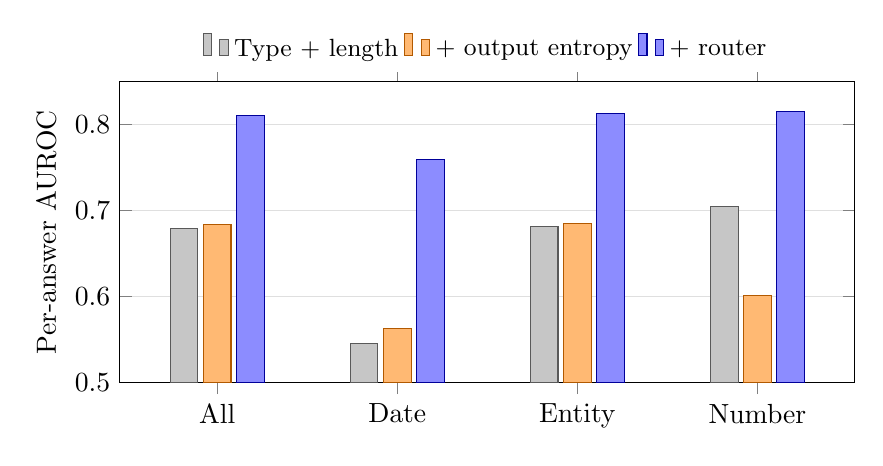
\begin{tikzpicture}
\begin{axis}[
  ybar, width=0.9\linewidth, height=5.4cm,
  ylabel={Per-answer AUROC},
  symbolic x coords={All,Date,Entity,Number},
  xtick=data, ymin=0.5, ymax=0.85,
  bar width=10pt, enlarge x limits=0.18,
  ymajorgrids, grid style={gray!25},
  legend style={at={(0.5,1.03)},anchor=south,legend columns=3,font=\small,draw=none}]
\addplot[fill=gray!45, draw=gray!70!black] coordinates {(All,0.679) (Date,0.545) (Entity,0.681) (Number,0.705)};
\addplot[fill=orange!55, draw=orange!70!black] coordinates {(All,0.684) (Date,0.563) (Entity,0.685) (Number,0.601)};
\addplot[fill=blue!45, draw=blue!60!black] coordinates {(All,0.811) (Date,0.759) (Entity,0.813) (Number,0.815)};
\legend{Type + length, + output entropy, + router}
\end{axis}
\end{tikzpicture}
\caption{Per-answer error detection on 1,792 non-arithmetic gpt-oss answers (cross-validated point estimates, no intervals). Output signals add almost nothing over question type and length; router statistics add 0.13 overall and 0.11 to 0.21 within each of the three largest types.}
\label{fig:response}
\end{figure}

No form of output entropy (mean, maximum, first token, sum, NLL, margin) beats length by more than 0.03, and added to type and length it contributes 0.005.
The router adds 0.13 over type and length, and it adds 0.11 to 0.21 within each of the three largest types (Figure~\ref{fig:response}).
These numbers come from one cross-validation without intervals.
The analysis also standardized the features on all 1,792 answers before splitting them into folds, which leaks their means and variances into the held-out folds.
A question-level bootstrap with standardization fitted inside each fold needs no new generation, only the saved features of this run, and we have not yet run it.
With that caveat, this is the measurement in this paper that most directly supports the starting hypothesis: the router carries information about errors that neither the output distribution nor surface covariates carry.

\subsection{Semantic entropy}
\label{sec:semantic}

We compare against semantic entropy~\citep{kuhn2023semantic,farquhar2024detecting} on 351 non-arithmetic test questions (69\% wrong), with five samples per question at temperature 0.8 clustered by meaning (equal numbers or overlapping words).
A first version of the clustering parsed ``560,000'' as 560 because of a locale-dependent number parser; after seeing the clusters we added a tolerant variant that compares the first number without separators, with 2\% tolerance and exact years.
We report both (Table~\ref{tab:semantic}).

\begin{table}[t]
\centering
\small
\caption{Per-answer AUROC on 351 non-arithmetic test questions (69\% wrong). The router detector was trained on train and calibration splits of the 2,600-question run.}
\label{tab:semantic}
\begin{tabular}{lcc}
\toprule
Signal & AUROC [95\% CI] & Generations \\
\midrule
Answer length & 0.660\ci{0.601}{0.720} & 1 \\
Router detector & \textbf{0.809}\ci{0.760}{0.855} & 1 \\
Semantic entropy, strict & 0.747\ci{0.690}{0.802} & 5 \\
Semantic entropy, tolerant & 0.757\ci{0.702}{0.808} & 5 \\
Router + semantic, tolerant & 0.833\ci{0.791}{0.875} & 6 \\
Cascade: semantic only on the 50\% most doubtful & 0.823 & 3.5 on average \\
\bottomrule
\end{tabular}
\end{table}

Semantic entropy's point estimate stays below the router's with five times the generation cost; the marginal intervals overlap, and we did not compute a paired difference for this comparison.
Adding it to the router gives $+0.024$\ci{-0.009}{+0.057} (tolerant) and $+0.014$\ci{-0.020}{+0.048} (strict), neither significant.
Our clustering is a string heuristic rather than the entailment model of the original method, so this comparison bounds a cheap implementation of semantic entropy, not the method in general.

\section{Replicating the InnerExpert protocol on OLMoE}
\label{sec:innerexpert}

The numbers above are not comparable with InnerExpert~\citep{fonseca2026innerexpert}: our labels are per answer, our prevalence is much higher, and our language is Spanish.
To compare directly, we ran our detector on InnerExpert's model and data: OLMoE-1B-7B-0924-Instruct, two answers per question (with and without evidence), greedy decoding up to 65 tokens, training on RealtimeQA 2024--2025 (2,318 questions), and testing out of distribution on RealtimeQA January--June 2026 (365 questions) and on 200-question samples of SQuAD~\citep{rajpurkar2016squad}, TruthfulQA~\citep{lin2022truthfulqa}, NQ-Open~\citep{kwiatkowski2019natural,lee2019latent}, and FreshQA~\citep{vu2024freshllms}, drawn with the same random seed as their pipeline.
Labels are spans marked by an LLM judge.
The judge rejected 89 of 6,966 answers (1.3\%) for format.

\begin{table}[t]
\centering
\footnotesize
\setlength{\tabcolsep}{3pt}
\caption{OLMoE-1B-7B on the InnerExpert protocol, token-level AUROC (1,000 bootstrap replicas). Our columns: this work; $\Delta$ is the paired difference between \FZO{} and output entropy. IE columns: published InnerExpert logistic-regression detector and logit-entropy baseline~\citep{fonseca2026innerexpert}. Prevalence is the share of hallucinated tokens in our test sets.}
\label{tab:innerexpert}
\begin{tabular}{lccccccc}
\toprule
Test set & Prev. & \FZO{} [95\% CI] & \FO{} & Entropy & $\Delta$ [95\% CI] & IE (LR) & IE entropy \\
\midrule
RealtimeQA 2026 & 40.9\% & 0.748\ci{0.729}{0.765} & 0.740 & 0.595 & $+0.154$\ci{+0.135}{+0.170} & 0.830 & 0.653 \\
SQuAD & 32.6\% & 0.650\ci{0.619}{0.682} & 0.632 & 0.603 & $+0.047$\ci{+0.016}{+0.079} & 0.787 & 0.650 \\
TruthfulQA & 27.3\% & 0.618\ci{0.582}{0.649} & 0.605 & 0.565 & $+0.052$\ci{+0.016}{+0.085} & 0.726 & 0.634 \\
NQ-Open & 32.6\% & 0.591\ci{0.558}{0.623} & 0.573 & 0.560 & $+0.031$\ci{-0.004}{+0.063} & 0.737 & 0.621 \\
FreshQA & 40.5\% & 0.649\ci{0.619}{0.678} & 0.643 & 0.532 & $+0.117$\ci{+0.088}{+0.144} & 0.732 & 0.636 \\
\midrule
Average & & \textbf{0.651} & 0.639 & 0.571 & $+0.080$ & 0.762 & 0.639 \\
\bottomrule
\end{tabular}
\end{table}

Our detector is 0.11 below InnerExpert on average and below it on every test set (Table~\ref{tab:innerexpert}).
Its advantage over output entropy is positive on all five sets but smaller: $+0.08$ on average against InnerExpert's $+0.12$.
The paired difference is significant on four sets and not on NQ-Open, where its interval is $[-0.004, +0.063]$.
The comparison is not exact, for four reasons:
\begin{enumerate}
  \item The judge is DeepSeek-v4-flash with our prompt, not GLM-5.1 with theirs. Our output-entropy baseline (0.571) is lower than theirs (0.639), which suggests that the labels differ.
  \item We run bf16 weights; the InnerExpert paper does not state the weight precision of its runs.
  \item We use only \FZ{} and \FO{}. InnerExpert adds expert-output similarity, expert hidden scores, and hidden-state and attention scores, which raise the cost of signal extraction to about $2.5\times$ plain generation~\citep{fonseca2026innerexpert}.
  \item We truncate the evidence at 10,000 characters; the published pipeline truncates the prompt from the right.
\end{enumerate}
We read this as a negative result for the router-only detector at equal protocol: the cheap router statistics recover part of the gain over entropy, and the expensive signals that we omit carry the rest.
Whether the gap is due to the omitted signals or to the label differences, we cannot separate with this run.

\section{Code generation}
\label{sec:code}

For code, a wrong answer is a program that fails its tests.
Most of its tokens are often correct, so a label copied to every token is a poor target.

\paragraph{Granite on HumanEval.}
Granite passes 58 of the 164 HumanEval~\citep{chen2021evaluating} tasks (35.4\%), fails 100, and errors on 6.
Token-level, the detector has no signal: 0.409\ci{0.239}{0.595} on 33 test answers (63.9\% error tokens), below output entropy (0.504\ci{0.447}{0.561}), which is itself at chance.
Per answer and without training, the mean router entropy reaches 0.74\ci{0.65}{0.82}, but answer length alone reaches 0.70 because failing solutions are longer, and length plus router reaches 0.735 under cross-validation.
Within length terciles, router entropy gives 0.61 to 0.76.
With 164 tasks and a 1B model, this is weak evidence.

\paragraph{gpt-oss-20b on HumanEval and MBPP.}
We added the 970 MBPP~\citep{austin2021program} tasks whose reference solution passes its own tests, for 1,134 tasks; gpt-oss passes 79.5\%.

\begin{table}[t]
\centering
\small
\caption{gpt-oss-20b on HumanEval and MBPP (1,134 tasks). Token-level rows use the test split (222 tasks; 22.5\% error tokens); per-answer rows use the 1,109 answers that contain code (207 failing). ``No training'' rows are single statistics averaged or maximized over the answer's tokens. Rows without an interval are cross-validated point estimates.}
\label{tab:code}
\begin{tabular}{lc}
\toprule
Measurement & AUROC \\
\midrule
Token-level, \FZO{} detector & 0.675\ci{0.551}{0.787} \\
Token-level, output entropy & 0.547\ci{0.516}{0.583} \\
Per answer, mean router entropy (no training) & 0.672\ci{0.629}{0.715} \\
Per answer, mean output entropy (no training) & 0.643\ci{0.603}{0.685} \\
Per answer, maximum output entropy (no training) & 0.648\ci{0.605}{0.692} \\
Per answer, length only & 0.592 \\
Per answer, CV: length + router entropy & 0.673 \\
Per answer, CV: length + output entropy & 0.634 \\
Per answer, CV: length + router entropy + output entropy & 0.673 \\
Per answer, CV: 243 router features + length & \textbf{0.758} \\
Per answer, mean output entropy over code lines (preregistered) & 0.555\ci{0.512}{0.598} \\
\bottomrule
\end{tabular}
\end{table}

On the larger model, the best per-answer predictor we found is the trained score on 243 router features plus length (0.758, a cross-validated point estimate; Table~\ref{tab:code}).
The untrained summaries are close to one another.
Mean router entropy reaches 0.672\ci{0.629}{0.715}, and mean output entropy over all answer tokens 0.643\ci{0.603}{0.685}; the intervals overlap, and we have no paired test.
Combined with length under cross-validation, router entropy gives 0.673 and output entropy 0.634, and output entropy adds nothing to length plus router entropy.
At the token level the detector's 0.675 and output entropy's 0.547 also have overlapping intervals.
A hypothesis written down from the Granite run before the gpt-oss data existed predicted that mean output entropy restricted to code lines (no docstrings or comments) would beat length; it scored 0.555 against 0.592 for length, so it is refuted (Appendix~\ref{app:rules}).
That restriction lowers output entropy from 0.643 to 0.555, so it is a poor variant, not the best output baseline.
As an alarm on single answers, the detector is weak: the $\alpha$ recommended on calibration (0.48) flags 85\% of failing solutions with 45\% false alarms.

\paragraph{Best-of-$N$.}
For code, ranking candidates is a more natural use than blocking one.
We trained the per-answer score on greedy answers to 887 train and calibration tasks and used it to choose one of five samples (temperature 0.8) for each of 213 test tasks; hidden tests only grade the choice.
The 887 are the train and calibration tasks (912 of the 1,134) whose greedy answer has a label and at least one code token; the 213 are the test tasks (of 222) that have a usable answer in all five sample runs.
We compare it with running the examples visible in the task statement, available for 190 of the 213 tasks (Table~\ref{tab:bestofn}).

\begin{table}[t]
\centering
\small
\caption{Best-of-5 selection on 213 gpt-oss test tasks. ``Examples'' first discards samples that fail the visible examples, then applies the policy.}
\label{tab:bestofn}
\resizebox{\linewidth}{!}{%
\begin{tabular}{lc@{\hspace{2em}}lccccc}
\toprule
Policy & Pass & Source & Random & Router & Ex.+random & Ex.+router & Oracle \\
\midrule
Random (expected) & 85.5\% & HumanEval ($n=39$) & 92.3\% & 92.3\% & 93.5\% & 94.9\% & 100\% \\
Shortest & 84.5\% & MBPP ($n=174$) & 84.0\% & 85.6\% & 88.1\% & 88.5\% & 91.4\% \\
Lowest code-line entropy & 85.4\% & & & & & & \\
Router score & 86.9\% & & & & & & \\
Examples + random & 89.1\% & & & & & & \\
Examples + router & \textbf{89.7\%} & & & & & & \\
Oracle (any passes) & 93.0\% & & & & & & \\
\bottomrule
\end{tabular}}
\end{table}

The router score beats the shortest sample by $+2.3$ points\ci{0.0}{+5.2}, at the edge of significance.
Running visible examples beats random by $+3.5$ points\ci{+2.0}{+5.3}, and adding the router on top of examples gives $+0.6$ points (we did not compute an interval for this difference).
Of the 7.5 points between random choice and the oracle, the free check with visible examples recovers 3.5 and the router adds little.
In MBPP the visible example is also one of the hidden tests, so part of that gain is mechanical; in HumanEval, where it is not, examples add only 1.2 points, and 39 tasks do not support a conclusion.
For code with executable examples, running the examples is the main action and the router is a tie-breaker.

\section{Cost of reading the signals}
\label{sec:latency}

The planned budget for the detector was less than 5\% added per-token latency (Appendix~\ref{app:rules}).
We measured it with interleaved A/B runs in the same process, fixed output lengths, and a paired overhead estimator: the median over (run, prompt) units of the ratio of per-token p50 latencies with and without hooks, with bootstrap intervals over units.

\paragraph{CPU.}
On a laptop CPU (i5-1035G1, 4 threads, Granite in bf16, 3 prompts $\times$ 4 interleaved runs, 24 tokens), p50 per-token latency rises from 280.6 to 303.2\,ms (+8.0\%) and mean time per output token from 331.6 to 359.8\,ms (+8.5\%); the paired estimate is +3.6\%\ci{-12.3\%}{+36.4\%}.
CPU latency on a laptop is too noisy (p95 of 1.5\,s per token) to accept or reject the budget.

\paragraph{HuggingFace on GPU.}
On a T4 (20 paired units, 5,100 per-token latencies), \FZO{} adds +3.00\%\ci{2.97\%}{3.03\%} and +0.57\% to the first token.
On an L4 (8 prompts $\times$ 5 runs, 256 tokens), the same code first added +7.6\%\ci{7.4}{7.9}, because the L4 generates faster and the fixed cost of Python hooks weighs more.
Profiling showed that the main per-token cost of \FZ{} was copying 201,088 logits to the CPU in float64.
After computing \FZ{} on the logits' device and converting router weights to float32 once per context, \FZ{} costs +1.0\%\ci{0.9}{1.1} and \FZO{} +4.7\%\ci{4.6}{4.8}, inside the budget with little margin.
A separate profile (6 prompts, 128 tokens, $n=18$ per variant) puts \FZO{} at +2.83\% and the same without the CPU-side reduction at +2.82\%: the reduction costs nothing measurable, and the remaining cost is in the hooks.
In gpt-oss the fused MXFP4 kernel does not call the router module, so a hook on that module never fires.
Our \FO{} hook therefore sits on the input of each MoE block and recomputes the router logits (Section~\ref{sec:method}); every HuggingFace cost above includes that recomputation.
Reading the logits that the kernel computes internally, which would avoid it, was not feasible.

\paragraph{vLLM.}
vLLM~\citep{kwon2023efficient} can return the indices of the routed experts with each token (\texttt{-{}-enable-\allowbreak return-\allowbreak routed-\allowbreak experts}), but not the router logits.
This supports the reduced tier of Section~\ref{sec:method}.
We used vLLM 0.31 on an L4.
The option requires restarting the server, so the latency with and without it comes from two separate server sessions, measured one after the other and not interleaved.
In each session we streamed 8 prompts $\times$ 3 runs of 256 tokens ($n=24$).
Median per-token latency is 22.57\,ms with the option and 22.61\,ms without it.
Pairing the 24 measurements by prompt and run, the median ratio is $-0.2\%$\ci{-0.4\%}{-0.2\%}, with a bootstrap over the 8 prompts.
That interval reflects variation across prompts only, not between server sessions, so we do not read it as a speed-up; one prompt was 23\% slower in the session without the option.
We read the result as no detectable cost.
Under 1 to 32 concurrent requests of code tasks (up to 256 tokens, two rounds per level, no interval), throughput through our proxy matches plain vLLM at every level (58 vs.\ 57 tokens/s at 1 request; 491 vs.\ 491 at 32).
Figure~\ref{fig:latency} summarizes the GPU measurements.

\begin{figure}[t]
\centering
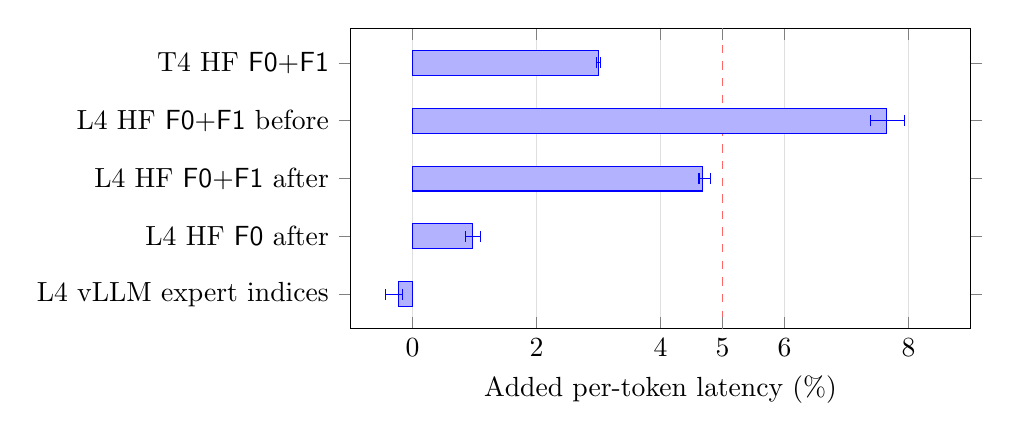
\begin{tikzpicture}
\begin{axis}[
  xbar, width=0.78\linewidth, height=5.4cm,
  xlabel={Added per-token latency (\%)},
  symbolic y coords={tfour,lbefore,lafter,lfzero,lvllm},
  ytick=data, y dir=reverse, xmin=-1, xmax=9,
  yticklabels={T4 HF \FZO{},L4 HF \FZO{} before,L4 HF \FZO{} after,L4 HF \FZ{} after,L4 vLLM expert indices},
  bar width=9pt, enlarge y limits=0.15,
  xmajorgrids, grid style={gray!25},
  extra x ticks={5}, extra x tick style={grid=major, grid style={dashed,red!60}},
  every axis plot/.append style={fill=blue!45, draw=blue!60!black}]
\addplot+[error bars/.cd, x dir=both, x explicit] coordinates {
  (3.00,tfour) += (0.03,0) -= (0.03,0)
  (7.64,lbefore) += (0.30,0) -= (0.25,0)
  (4.68,lafter) += (0.12,0) -= (0.06,0)
  (0.97,lfzero) += (0.13,0) -= (0.12,0)
  (-0.23,lvllm) += (0.07,0) -= (0.20,0)};
\end{axis}
\end{tikzpicture}
\caption{Added per-token latency on GPU. The dashed line is the 5\% budget. ``Before'' and ``after'' refer to moving output features to the logits' device and converting router weights once per context. The vLLM bar is the median ratio of per-token latency with and without returning expert indices, paired by prompt and run ($n=24$), with a bootstrap interval over 8 prompts; the two conditions ran in separate server sessions, so the interval omits between-session variation.}
\label{fig:latency}
\end{figure}

\paragraph{How much signal survives in vLLM.}
On the 600-question set served through vLLM (59.3\% correct; arithmetic always correct), the global token-level AUROC of 0.947 mostly measures question type.
Within MKQA, with the detector retrained on a fresh 60/20/20 split of the stratum (66 test questions), the vLLM tier reaches 0.784\ci{0.639}{0.916}, against 0.512\ci{0.396}{0.644} for its output features alone and 0.461 for token NLL.
The paired differences are $+0.272$\ci{+0.153}{+0.382} against its output features and $+0.322$\ci{+0.196}{+0.425} against token NLL.
The stratum is small, and the number depends on the split: the same stratum evaluated on the questions of the global split gives 0.895.
The full HuggingFace tier reached 0.837 in the T4 run of Table~\ref{tab:gptoss}, a different run.
Offline, on the 1,792 factual answers of Section~\ref{sec:response}, adding vLLM-available features to type and length gives 0.742 per answer, against 0.679 without them and 0.811 with full router logits (point estimates): expert indices keep about half of the per-answer gain.
In the same L4, vLLM generates at about 22.6\,ms per token and HuggingFace at 76.7\,ms, under different protocols.

\section{Discussion}
\label{sec:discussion}

\paragraph{What the router adds.}
Across three MoE families and two languages, router statistics have a higher AUROC than output entropy on every factual comparison, including within the three largest question types and on out-of-distribution test sets.
The paired difference is significant wherever we could compute it, except on NQ-Open; for the gpt-oss runs only marginal intervals are available.
On code, the router's point estimates are above output entropy's on gpt-oss-20b with overlapping intervals, and the router fails with Granite at the token level.
Per answer, router statistics add information that neither length, question type, nor any summary of the output distribution carries, by point estimate.
This agrees with InnerExpert and Routing Entropy on the direction of the effect~\citep{fonseca2026innerexpert,li2026routing}, and contrasts with the null result of \citet{liang2026auditing} in vision transformers, where routing entropy was audited against a strong output-only baseline; in our language models the output-only baseline is weak, and on most test sets the router's margin over it is wide.

\paragraph{What it does not add.}
The router does not clearly beat a linear probe on the late hidden state in any setting where we could run both.
They tie on Granite (0.906 each; paired difference $0.000$\ci{-0.032}{+0.036}); the router is ahead by 0.010 on the gpt-oss T4 run and behind by 0.020 on the 2,600-question run, where only marginal intervals are available and they overlap widely (Tables~\ref{tab:granite}, \ref{tab:strata}, \ref{tab:gptoss}).
Our results therefore do not support a claim that routing contains information beyond the hidden state; they support the narrower claim that a compact, cheap, already-computed summary recovers most of what a hidden-state probe recovers.
That summary has practical value: it is 243 numbers per token, it does not require choosing a probe layer, and in vLLM a reduced version arrives with the tokens at no detectable cost.
It does not match a richer MoE detector on that detector's own protocol.

\paragraph{How to report router detectors.}
Three measurement choices moved our headline numbers more than any modeling choice.
Prevalence and answer-type mix: the 0.906 on Granite comes from a test where 92\% of tokens are errors and arithmetic is much easier than MKQA; pooling the non-arithmetic types of a larger set gives 0.72.
Label granularity: copying an answer label to all its tokens turns token-level AUROC into a smoothed answer-level metric, and it fails outright for code, where a wrong program is mostly right.
Covariates: length predicts errors on its own (0.67 per answer on factual questions, 0.70 on Granite code), so a router detector should be compared with length and type, not only with entropy.
We suggest that work on internal error signals report within-type results, prevalence, a length baseline, and paired intervals for differences alongside global AUROC; we did not keep paired intervals for every run ourselves.

\paragraph{What to use, by task.}
The measurements point to different actions for different tasks.
For short factual answers, the most useful single signal we found is a per-answer score built from router statistics together with question type and answer length (Table~\ref{tab:response}); it needs one generation, and its point estimate is above five-sample semantic entropy in our implementation, with overlapping intervals (Table~\ref{tab:semantic}).
As a per-token alarm on the same answers, the detector is usable but not precise: at the recommended $\alpha$ it catches 86\% of wrong answers and raises an alarm on 27\% of right ones, on a test split where more than half of the right answers are arithmetic (Appendix~\ref{app:pareto}).
Whether that trade-off is acceptable depends on the cost of a missed error relative to a false alarm, which conformal risk control lets an operator set through $\alpha$ but not escape.
For code with executable examples, the first action is to run the examples; the router helps only to break ties among candidates that pass them (Table~\ref{tab:bestofn}).
As a single-answer alarm for code, the detector is too weak to use (85\% recall at 45\% false alarms).
For serving, the HuggingFace tier fits a 5\% latency budget on an L4 only after moving output features to the GPU, and the margin is small.
In vLLM, returning expert indices has no detectable cost, and the reduced tier keeps most of the within-type token-level signal and about half of the per-answer gain; an engine that also returned router logits would remove that loss.

\paragraph{Why a cheap summary may be enough.}
The router of each MoE layer is a linear map of the hidden state entering that layer, followed by a softmax.
Its logits are therefore a low-dimensional projection of the residual stream at every layer, learned to separate the inputs that different experts handle.
It is not surprising that such projections, taken across 24 layers and summarized by entropy, margins and usage, recover most of what a probe on one late layer recovers.
This reading also explains the two failures.
A router projection cannot see an error that the hidden state does not encode, so it cannot beat the probe; and a router-only detector omits the expert outputs and attention scores that InnerExpert adds, which is where we expect most of its remaining advantage to lie.
We have not tested this explanation directly.

\section{Limitations}
\label{sec:limits}

\begin{itemize}
  \item Factual labels are per answer, not per span. Only the OLMoE replication uses span labels, and those come from an LLM judge that we did not validate against humans.
  \item The base set is small (120 test questions), and Granite's 92\% error rate makes its intervals wide and its flag rates uninformative.
  \item The main factual experiments use Spanish MKQA questions and generated arithmetic; the English results come only from the replication.
  \item We tested three MoE models up to 20B parameters. We did not run gpt-oss-120b.
  \item The router never clearly beat the hidden-state probe. We did not test whether router features transfer across domains or models better than a probe.
  \item In a companion study~\citep{companion2026forgetting}, we asked whether the Granite instruct detector, without output features, tracks how certain the model is of a stored fact. In the base model, on 461 UniEdit facts~\citep{chen2025uniedit}, its doubt correlates with the loss of the fact's value with Spearman $+0.079$ (90\% CI $[+0.001, +0.155]$). A router-only probe trained on the base model separates the facts the model knows from the rest, among the 379 facts that have that label, with AUROC 0.591 (90\% CI $[0.541, 0.637]$). In the instruct model the result repeats (Spearman $+0.059$, 90\% CI $[-0.019, +0.134]$, 461 facts; AUROC 0.598, 90\% CI $[0.550, 0.645]$, 379 facts). These intervals come from a bootstrap over facts at the 90\% level fixed in that study's preregistration. The router detects erroneous tokens during generation, but it does not read how certain the model is of a fact.
  \item Semantic entropy used a string-matching clustering heuristic, and its tolerant variant was added after inspecting clusters.
  \item The InnerExpert replication differs in judge, feature set, and truncation, and possibly in weight precision.
  \item Paired differences are available only for the Granite base set, the OLMoE replication and the vLLM run. For the gpt-oss runs on HuggingFace we kept marginal intervals only, and the per-answer results of Section~\ref{sec:response} have no interval yet.
  \item Latency on CPU was too noisy to decide. HuggingFace latency depends on hook overhead, which differs between GPUs; the vLLM tier lacks router logits, and its latency comparison comes from two server sessions that were not interleaved.
  \item Most analyses were not preregistered. Appendix~\ref{app:rules} lists the two decision rules that were written before the data, and the post-hoc changes we made.
\end{itemize}

\section*{Reproducibility}
[CODE AND DATA AVAILABILITY: repository URL, datasets, detector artifacts, and evidence files.]
The Granite experiment runs with one command on a laptop CPU in about two hours:
\begin{verbatim}
python -m vigia.cli evidence \
  --model ibm-granite/granite-3.1-1b-a400m-instruct --dtype bfloat16 \
  --data evidence_v1.jsonl --out runs/evidence_v1 --max-tokens 24 \
  --tiers F0,F1,H --n-boot 2000 --bench 4
\end{verbatim}
The run is resumable. The GPU experiments run from scripts for Colab in the same repository.
They use HuggingFace Transformers for the hooked runs and vLLM 0.31 for the serving runs; generation limits are 24 (Granite) and 256 (gpt-oss) new tokens for factual answers and 384 (Granite) and 768 (gpt-oss) for code.
The paired differences reported in this version are recomputed from the saved evaluation reports and features by one script in the repository.

\section*{Acknowledgments}
The experiments were designed, run, and written up with the help of an AI coding assistant (Claude); the author takes responsibility for all content.

\bibliographystyle{plainnat}
\bibliography{refs}

\appendix
\section{Pre-specified rules and outcomes}
\label{app:rules}

Unlike the companion paper~\citep{companion2026forgetting}, the detector work did not keep a preregistration log for every run.
Two rules were written down before the data that tested them; Table~\ref{tab:rules} lists them with their outcomes.

\begin{table}[h]
\centering
\scriptsize
\caption{Rules written before the data that tested them. ``Pass'' and ``fail'' refer to the rule as written.}
\label{tab:rules}
\begin{tabular}{p{2.6cm}p{5.6cm}p{5.6cm}}
\toprule
Experiment & Rule & Result \\
\midrule
Stage-1 gate (project plan) & On gpt-oss-20b, the router signal beats output entropy, with less than 5\% added latency & pass on T4 (0.881 vs.\ 0.643, non-overlapping marginal intervals; +3.0\%); fail on L4 at first (+7.6\%); pass on L4 after optimization (+4.7\%); pass in vLLM (no detectable cost) \\
Code, from Granite to gpt-oss & Mean output entropy over code lines predicts failure better than length (Granite: 0.79 vs.\ 0.71); router entropy loses its signal under the same filter (Granite: 0.74 $\rightarrow$ 0.56) & fail, 0.555 vs.\ 0.592 for length; partial for the router, 0.672 $\rightarrow$ 0.614 \\
\bottomrule
\end{tabular}
\end{table}

Post-hoc changes: the tolerant number parser for semantic entropy was added after inspecting clusters, and both variants are reported; the L4 latency code was optimized after the first L4 measurement failed the budget, and both measurements are reported; the InnerExpert replication switched judge because the original judge's account ran out of credit.
An earlier CPU latency run was discarded because other processes saturated the CPU.
The vLLM measurement exposed two defects in our proxy, both fixed before the reported run: vLLM returns routed experts as base64-encoded \texttt{.npy} arrays that include prompt rows, and gpt-oss log-probabilities include the \texttt{analysis} channel.

\section{Flagging trade-offs}
\label{app:pareto}

Table~\ref{tab:pareto} shows, for the 2,600-question gpt-oss run, the answer-level detection and false-alarm rates on test as a function of $\alpha$, where an answer is flagged if any of its tokens is flagged.
The test split has 241 wrong and 237 right answers; all wrong answers are non-arithmetic, and 127 of the right answers are arithmetic.
The recommended $\alpha$ maximizes detection minus false alarms on the calibration split, with ties broken toward the smaller $\alpha$.

\begin{table}[h]
\centering
\small
\caption{Answer-level trade-off on the gpt-oss 2,600-question test split, all question types pooled. The recommended $\alpha$ is chosen on the calibration split.}
\label{tab:pareto}
\begin{tabular}{ccc}
\toprule
$\alpha$ & Wrong answers flagged & Right answers flagged \\
\midrule
0.10 & 96\% & 43\% \\
0.20 & 90\% & 32\% \\
0.26 (recommended) & 86\% & 27\% \\
0.34 & 81\% & 22\% \\
0.42 & 76\% & 16\% \\
0.50 & 74\% & 15\% \\
\bottomrule
\end{tabular}
\end{table}

For code, the recommended $\alpha$ (0.48) flags 85\% of failing solutions and 45\% of passing ones on 41 failing and 181 passing test tasks.

\end{document}
